%% BEAMER slides (with notes)
%
%
\documentclass[a4paper,12pt]{beamer}
\usepackage{graphicx}
\usepackage{amsmath}
\usepackage{amssymb}
\usepackage{bm}
\usepackage{tikz}
\usepackage{pgfplots}
\title{Approximating price vectors for price discrimination over networks}
\date{\today}
\author{Calvin Roth}
\usetheme{Madrid}
\begin{document}
\maketitle

\tableofcontents
\section{Introduction}
\begin{frame}{Motivation}
  \begin{itemize}
    \item Humans are social creatures, our behavior influences other behavior
    \item When our peers engage in a behavior, we are more likely do so as well
    \item This behavior is widespread from promoting exercise\cite{SocialInfluenceandExerciseAMetaAnalysis}, modeling likelihood to smoke\cite{urberg1997close} or purchase environmentally green products\cite{dagher2012influence}
  \end{itemize}
\end{frame}

\begin{frame}{Motivation}
  \begin{itemize}
    \item Provide a mathematical framework that incorporates social influence to provide guidance to marketers and policy designers \\
 \item We will use the model first proposed by~\cite{candogan2012optimal} and later used by~\cite{huang2021value} to model an individuals utility u
          \begin{equation}
            u_{i}(x, p) = ax_{i} - x_{i}^{2} + 4 \rho x_{i} \sum \frac{G_{ij}}{\|G+G^{T}\|} x_{j} - p_{i}x_{i}
          \end{equation}
          where $a,\rho$ are constants and $p_{i}$ is the price user i is charged.
\end{itemize}
\end{frame}


\begin{frame}
  \begin{itemize}
    \item A manufacturer who can produce goods at unit cost c with $c < a$ wants to maximize profits.
    \item Use network information to charge influencers less and influencees more.
    \item The optimal prices to charge each individual when the network is fully known is well understood\cite{candogan2012optimal}\cite{huang2021value}

          \begin{equation}
            \frac{a+c}{2} \textbf{1} + \frac{a-c}{2} \frac{\rho}{\| G + G^{T}\|} (G - G^{T}) K(G+G^{T}, \frac{\rho}{\|G+G^{T}\|})
          \end{equation}
          where $K(X, y) = {(I - yX)}^{-1}\textbf{1}$, the Bonacich centrality vector.
          \item This vector is a weighted sum of walks ending at vertex i.
   \end{itemize}
\end{frame}

\begin{frame}
  \begin{itemize}
    \item But we often don't have ready access to the full network information
    \item Given partial enough of the network ex.\ degrees of network what should we do?
    \item Specifically, we want a way to generate a ``good enough'' price vector v with respect to this partial information
          Goal: minimize expected regret
          \begin{equation}
            \mathbb{E} [ 1 - \frac{P_{G}(v)}{Optimal\-Profit} | \text{Statistic of G}]
          \end{equation}
          Where $P_{G}(v)$ is the profit of our v applied to the real network G.
  \end{itemize}
\end{frame}


\begin{frame}
  \frametitle{Degree Seqeunce Information}
  \begin{itemize}
    \item Suppose we are given the degree sequence of the network G (directed graph)
    \item Strategy 1: Make a new graph H with the same degree sequence as G using the configuration model
    \item Hypothesis: H behaves like G so maybe the optimal price vector of H is close to the optimal price vector of G
          \item It is not obvious that local properties of the network should strongly impact global properties (optimal profit)
  \end{itemize}
\end{frame}

\begin{frame}
  \frametitle{Overview of the results}
  \begin{itemize}
    \item The answer is yes, this is a strategy to get good price vectors for an unknown graph \\
    \item The following results will show this to be the case
  \end{itemize}
\end{frame}

\begin{frame}
  \frametitle{Details of Testing}
  \begin{itemize}
    \item Generate a graph G with the Erdos-Renyi model with n nodes and link probablity p
    \item Generate either Same Parameter graphs (i.e.\ same n and p but no further restriction) or Graphs with the same sequence
    \item After we have generated a price vector use G to check how close we were.
    \item For fixed G, get the average regret over several runs
  \end{itemize}
\end{frame}

\section{Regret of Profits}
\begin{frame}
  \frametitle{Distribution of profit regret}
  \begin{itemize}
    \item How much regret would we have if we used the optimal same sequence price vector or the same parameter price vector. Lower is better
        \item Using graphs of the same sequence outperforms all Erdos-Renyi Graphs of the same n and p.
    \item $n=1500, p \in [\frac{1}{n}, \frac{log(n)}{n}]$
  \end{itemize}
  \includegraphics[width=0.6\textwidth]{results/RegretVP.png}
  %\includegraphics[width=0.59\textwidth]{results/profit_regret.png}
\end{frame}

\begin{frame}{As a function of n}
  \begin{itemize}
    \item $n \in [100, 3000], p = \frac{\sqrt{\log(n)}}{n}$
  \end{itemize}
  \includegraphics[width=0.8\textwidth]{results/profit_regret.png}
\end{frame}

\begin{frame}{What about the raw profits}
  \begin{itemize}
    \item Raw profit holds little meaning as the optimal profit will change a lot with changes to p and n \\
  \end{itemize}

  \includegraphics[width=0.8\textwidth]{results/profit_dist.png}
  \end{frame}

\begin{frame}
  \frametitle{Statistic of distribution of Profits}
  \begin{itemize}
    \item Mean Profit of all same parameter Erdos Renyi graphs: 457.369\\
    \item Variance of same parameter case: 14.377
    \item Mean Profit of same sequence profits 489.190
    \item Variance of same sequence profits 0.008
    \item True Optimal Profit 490.030
  \end{itemize}
\end{frame}


\section{Errors in prices}
\begin{frame}
  \frametitle{Distribution of Prices}
  \begin{itemize}
    \item The next question to ask is do the same sequence price vectors look like the optimal price vector?
    \item Again the answer is yes
  \end{itemize}
\end{frame}

\begin{frame}
  \frametitle{Average  differences in price }
  \begin{itemize}
    \item Generate fixed G and find true optimal price vector $v_{opt}$
    \item Generate a guess of a graph and its price vector $v_{guess}$
    \item $score = \frac{1}{(\# Trials)*n}\sum_{\# Trials} \| v_{opt} - v_{guess}\|_{1} $
    \item Average error in each price.
    \item Same for $\ell_{2}$
  \end{itemize}
\end{frame}

\begin{frame}
  \frametitle{$\ell_{1}$ Difference}
  $p=\frac{\sqrt{\log(n)}}{n}$
  \includegraphics[width=0.8\textwidth]{results/price_vector_l1.png}
\end{frame}

\begin{frame}
  \frametitle{$\ell_{2}$ Difference}
  \includegraphics[width=0.8\textwidth]{results/price_vector_l2.png}
\end{frame}

\begin{frame}
  \frametitle{$\ell_{\infty}$ Difference}
  Simpler formula $\frac{1}{\# Trials} \sum_{Trials} \| v_{true} - v_{guess} \|_{\infty}$
  \includegraphics[width=0.8\textwidth]{results/price_vector_inf.png}
\end{frame}

\begin{frame}{Effect of p}
  \begin{itemize}
    \item $n=1500, p \in [\frac{1}{n}, \frac{\log(n)}{n}]$
    \item No clear effect of p on error in price
  \end{itemize}
  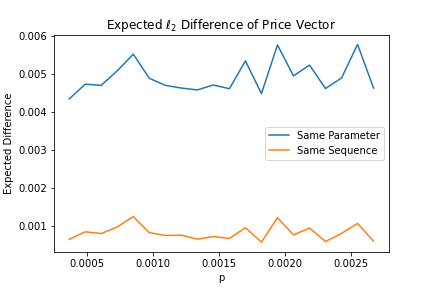
\includegraphics[width=0.4\textwidth]{results/vdif_vp_l2.png}
  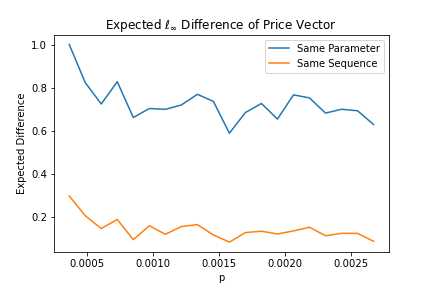
\includegraphics[width=0.4\textwidth]{results/vdif_vp_inf.png}
\end{frame}

\begin{frame}{Differences in Price Vector}
  \begin{itemize}
    \item The price vector from the same sequence graphs is always notably closer than for the same parameter graph \\
    \item For the same parameter graphs $\ell_{2}$ norm appears to converge but $\ell_{\infty}$ appears stagnant regardless of the size of the network.
  \end{itemize}
  \end{frame}

\section{A second strategy}
\begin{frame}
  \frametitle{A second strategy}
  \begin{itemize}
    \item Above we have shown that the price vector of generated graphs is on average like the optimal price vector\\
    \item {\color{blue}Strategy 2} The averaged price vector is even close to the optimal price vector
          \begin{equation}
            v = \frac{1}{\# Trials} \sum Profit_{G} (\text{Guessed vector})
          \end{equation}
          \begin{equation}
            v = Profit_G ( \frac{1}{\# Trials} \sum \text{Guessed vector} )
          \end{equation}
  \end{itemize}
\end{frame}

\begin{frame}
  \frametitle{Results}
  Comparison between these two strategies: $p=\frac{\sqrt{\log(n)}}{n}$
  \includegraphics[width=0.8\textwidth]{results/RegretAveragedVector.png}
\end{frame}

\begin{frame}
  \frametitle{Results}
  Conjecture ratio of these two regrets appear to approach Strategy 2 is twice as good as Strategy 1
  \includegraphics[width=0.8\textwidth]{results/ratio_regret_avg_vector_diff.png}
\end{frame}

\section{Walk Size}
\begin{frame}
  \frametitle{Other Directions}
  \begin{itemize}
    \item If knowing the degrees is good then maybe knowing $\left[|N(v)|, |N(N(v))\setminus (N(v) \cup v ) |\right]$ is better\\
    \item i.e.\ how many nodes can v reach in 1 or 2 steps \\
    \item What about k steps?
  \end{itemize}
\end{frame}

\begin{frame}
  \frametitle{Walk Test}
  \begin{itemize}
    \item Instead of calculating ${(I - \frac{\rho}{\| G + G^{T}\|}(G+G^{T}) )}^{-1} \textbf{1}$ we calculate $\sum_{i=1}^{k} {( \frac{\rho}{\|G+G^{T}\|} (G+G^{T}) )}^{k}$ \\
    \item I.e.\ only walks of length k or less have any bearing on the price vector \\
  \end{itemize}
\end{frame}

\begin{frame}
  \frametitle{Results}
  The loss from number of steps decays very quickly at first then marginal utility.\ n=1000
  \includegraphics[width=0.8\textwidth]{results/walk_loss.png}
\end{frame}

\section{Next Steps}
\begin{frame}{Next Steps}
  \begin{itemize}
    \item Derive mathematical bounds \\
    \item Explore other network configurations other than Erdos-Renyi \
    \item Possibility of more sophisticated pricing vectors
  \end{itemize}
\end{frame}

\bibliography{refer}
\bibliographystyle{ieeetr}

\end{document}

